\documentclass[11pt]{article}
\usepackage[cm]{fullpage}
%%AVC PACKAGES
\usepackage{avcgreek}
\usepackage{avcfonts}
\usepackage{avcmath}
\usepackage[numberby=section]{avcthm}
\usepackage{qcmacros}
\usepackage{goldstone}
%%MACROS FOR THIS DOCUMENT
\numberwithin{equation}{section}
\usepackage[
  margin=1.5cm,
  includefoot,
  footskip=30pt,
  headsep=0.2cm,headheight=1.3cm
]{geometry}
\usepackage{fancyhdr}
\pagestyle{fancy}
\fancyhf{}
\fancyhead[LE,RO]{Quiz 1, Handout 1: Hartree-Fock}
\fancyfoot[CE,CO]{\thepage}
\usepackage{url}

\begin{document}

\section{Hartree-Fock Theory}

The goal of electronic structure theory is to solve the ``clamped-nuclei'' Schr\"odinger equation
\begin{align}
\label{eq:electronic-schrodinger-equation}
  \op{H}\Y_k
=&\
  E_k\Y_k
&
  \op{H}
=&\
  V_{\mr{nuc}}
+
  \op{H}_e
=
  \sum_{a<b}^{\text{nuc.}}
  \fr{Z_aZ_b}{|\bo{R}_a-\bo{R}_b|}
-
  \fr{1}{2}
  \sum_i^{\text{elec.}}
  \nabla_i^2
-
  \sum_a^{\text{nuc.}}
  \sum_i^{\text{elec.}}
  \fr{Z_a}{|\bo{R}_a-\bo{r}_i|}
+
  \sum_{i<j}^{\text{elec.}}
  \fr{1}{|\bo{r}_i-\bo{r}_j|}
\end{align}
with an optimal balance of accuracy and efficiency for the problem of interest.
The most accurate solution possible for a given atomic orbital (AO) basis set\footnote{cc-pVXZ, 6-31G, ANO1, etc.} results from expanding the wavefunction
\begin{align}
\label{eq:full-ci-wavefunction-expansion}
  \Y_k
=&\
  \sum_\mu
  \F_\mu c_{\mu k}
\end{align}
in terms of all possible Slater determinants $\F_\mu$ that can be formed from an orthonormal one-electron basis of spin-orbitals, $\{\y_p\}$.
The expansion coefficients $(\bo{c})_k=c_{\mu k}$ are eigenvectors of the matrix $(\bo{H})_{\mu\nu}=\ip{\F_\mu|\op{H}|\F_\nu}$, which is the matrix representation of the Hamiltonian in the determinant basis.
This is called the {\it full configuration-interaction}\ (FCI) solution.

Any one-electron basis spans the same ``function space'' as the AO basis set itself, and the full $n$-electron basis $\{\F_\mu\}$ spans the same space of $n$-electron functions regardless of how one forms spin orbitals from the AO basis set.
As a result, one obtains the same FCI solution for any choice of spin-orbitals.
In general, however, FCI solutions are completely unfeasible for basis sets of sufficient size to approach the complete basis set limit.
One can think of this as a simple counting problem: if there are $m$ functions in the AO basis, then there are $2m$ spin-orbitals in the one-electron basis,\footnote{$m$ $\a$-orbitals and $m$ $\b$-orbitals.} and there are ``$2m$ choose $n$''\footnote{The number of unique sets of $n$ marbles that can be drawn from a bag of $2m$ marbles. See \url{http://en.wikipedia.org/wiki/Combination}}
\begin{align*}
{2m \choose n}\equiv\fr{(2m)!}{n!(2m-n)!}
\end{align*}
unique Slater determinants in the $n$-electron basis that can be formed from the spin MOs.
The upshot is that we usually have to omit some Slater determinants in order to get an answer in a reasonable amount of time.

As soon as we truncate our determinant expansion (\ref{eq:full-ci-wavefunction-expansion}), our choice of spin MOs makes a significant difference in the quality of our results.
In particular, we need to choose our set of one-electron functions to minimize the number of Slater determinants it takes to ``get close to'' the exact wavefunction.


\subsection{The Hartree-Fock optimization problem}

It can be shown that optimizing $\ip{\Y|\op{H}_e|\Y}$ by varying $\Y$ subject to the normalization constraint $\ip{\Y|\Y}=1$ is equivalent to solving the Schr\"odinger equation.
When we further constrain the form of $\Y$ this is no longer true, but it \textit{does} generally allow us to get the best approximation to $\Y$ for a given approach (or ``Ansatz'').

In order to make the wavefunction expansion converge with a relatively small number of $\F_\mu$s, we wish to find the best single-determinant approximation to $\Y$.
That is, we wish to optimize
\begin{align}
  \ip{\F|\op{H}_e|\F}
\sp\sp
  \F(1,\ld,n)
=
\fr{1}{\sqrt{n!}}
\left|\ar{%
  \y_1(1)&\y_2(1)&\cd&\y_n(1)\\
  \y_1(2)&\y_2(2)&\cd&\y_n(2)\\
  \vd    &\vd    &\dd&\vd    \\
  \y_1(n)&\y_2(n)&\cd&\y_n(n)}\right|
\end{align}
with respect to variation of the orbitals $\{\y_p\}$, enforcing the normalization constraint by keeping the spin orbitals orthonormal.
Note that here the function argument $(i)$ is shorthand for $(\bo{r}_i,s_i)$ where $\bo{r}_i$ denotes the position of the $i\eth$ electron and $s_i$ denotes its spin.
This optimization problem is the idea behind \textit{Hartree-Fock theory}.

Once we have solved for the Hartree-Fock optimization problem, the expectation value $\ip{\F|\op{H}_e|\F}$ is itself a good first approximation to the electronic energy.
More importantly, however, when we use this new set of Hartree-Fock spin-orbitals, $\{\y_p\}$, the FCI expansion tends to converge much more quickly to the true wavefunction.
Specifically, when we rewrite equation~\ref{eq:full-ci-wavefunction-expansion} in terms of single $\{\F_i^a\}$, double $\{\F_{ij}^{ab}\}$, triple $\{\F_{ijk}^{abc}\}$, etc.\ replacements\footnote{It is typical to use dummy indices $i,j,k,l$ to count over the orbitals in the reference determinant $\F$ -- the ``occupied orbitals'' -- and to use $a,b,c,d,$ to count over the orbitals not contained in $\F$ -- the ``unoccupied'' or ``virtual orbitals.''  Dummy indices $p,q,r,s$ are generally used to count over the full set of spin-orbitals, whether occupied or not.} of the orbitals in the Hartree-Fock determinant $\F$ with the remaining orbitals in the basis
\begin{align}
  \Y
=
  \F
+
  \sum_{\substack{a\\i}}
  \F_i^ac_a^i
+
  \sum_{\substack{a<b\\i<j}}
  \F_{ij}^{ab}c_{ab}^{ij}
+
  \sum_{\substack{a<b<c\\i<j<k}}
  \F_{ijk}^{abc}c_{abc}^{ijk}
+\ld
\end{align}
the coefficients tend to be very small, and are often virtually negligible for higher than quadruple replacements.

\subsection{The Hartree-Fock equations}

The electronic Hamiltonian $\op{H}_e$ contains one- and two-electron operators.
\begin{align}
  \op{H}_e
=&\
  \sum_i
  \op{h}(i)
+
  \sum_{i<j}
  \op{g}(i,j)
&
  \op{h}(i)
&\equiv
-
  \fr{1}{2}
  \nabla_i^2
+
  \sum_a
  \fr{Z_a}{|\bo{r}_i-\bo{R}_a|}
&
  \op{g}(i,j)
&\equiv
  \fr{1}{|\bo{r}_i-\bo{r}_j|}
\end{align}
Its expectation value with respect to a single determinant $\F$ is given by the first Slater rule
\begin{align}
\label{eq:slater-rule-1}
  \ip{\F|\op{H}_e|\F}
=
\sum_{i}^n
  \ip{\y_i|\op{h}|\y_i}
+\fr{1}{2}\sum_{ij}^n
  \ip{\y_i\y_j||\y_i\y_j}
&&
  \ip{\y_p\y_q||\y_r\y_s}
\equiv
  \ip{\y_p\y_q|\y_r\y_s}
-
  \ip{\y_p\y_q|\y_s\y_r}
\end{align}
where the one- and two-electron integrals are defined as follows.
\begin{align}
\label{eq:one-and-two-electron-integrals}
  \ip{\y_p|\op{h}|\y_q}
\equiv&\
  \int
  d(1)
  \y_p^*(1)
  \op{h}(1)
  \y_q(1)
&
  \ip{\y_p\y_q|\y_r\y_s}
\equiv&\
  \int
  d(1)d(2)
  \y_p^*(1)\y_q^*(2)
  \op{g}(1,2)
  \y_r(1)\y_s(2)
\end{align}
We wish to optimize equation~\ref{eq:slater-rule-1} while constraining the orbitals to be normalized and orthogonal.\footnote{The $\overset{!}=$ sign means ``must equal'' -- these are conditions to be satisfied.}
\begin{align}
  \ip{\y_i|\y_j}
\overset{!}{=}
  \d_{ij}
\end{align}
The corresponding Lagrangian functional (see \cref{app:constrained-optimization}) is
\begin{align}\label{eq:hartree-fock-lagrangian}
  \mc{L}[\{\y_i\},\{\y_i^*\},\{\ev_{ij}\}]
=
  \sum_{i=1}^n
  \ip{\y_i|\op{h}|\y_i}
+
  \fr{1}{2}
  \sum_{i,j=1}^n
  \ip{\y_i\y_j||\y_i\y_j}
-
  \sum_{i,j=1}^n
  \ev_{ij}(\ip{\y_i|\y_j}-\d_{ij})
\end{align}
where $\{\ev_{ij}\}$ are our Lagrangian multipliers for the orthonormality constraint.
Note that the complex conjugates of the orbitals $\{\y_i^*\}$ are included as separate arguments of $\mc{L}$, since the real and imaginary components of $\y_i$ can be varied independently.\footnote{One can explicitly show that for complex variables $\dpd{z}{z^*}=0$.  See \url{https://en.wikipedia.org/wiki/Wirtinger_derivatives#Functions_of_one_complex_variable}.}

The stationarity conditions for the Hartree-Fock Lagrangian are (see \cref{app:functional-derivatives})
\begin{align}\label{eq:hartree-fock-lagrangian-stationarity}
\left.
  \fr{d\mc{L}[\y_k^*+\e \h^*]}{d\e}
\right|_{\e=0}
\overset{!}=
  0
\hspace{10pt}
  \text{and}
\hspace{10pt}
\left.
  \fr{d\mc{L}[\y_k+\e \h]}{d\e}
\right|_{\e=0}
\overset{!}=
  0
\hspace{10pt}
  \text{for all $\h$}
&&
  k=1,\ld,n
\end{align}
which can be stated in words as follows: For each orbital $\y_1,\ld,\y_n$ in the determinant $\F$, mixing in a little bit of an arbitrary function $\eta=\eta(\bo{r},s)$ doesn't change the Lagrangian.

Separating out the terms in \cref{eq:hartree-fock-lagrangian} involving a particular orbital $\y_k$, we can write
\begin{align*}
  \mc{L}
=&\
  \ip{\y_k|\op{h}|\y_k}
+
  \sum_i
  \ip{\y_k\y_i||\y_k\y_i}
-
  \sum_i
  \ev_{ki}(\ip{\y_k|\y_i}-\d_{ki})
-
  \sum_i
  \ev_{ik}(\ip{\y_i|\y_k}-\d_{ik})
\\&\
+
  \sum_{i\neq k}
  \ip{\y_i|\op{h}|\y_i}
+
  \fr{1}{2}
  \sum_{i\neq k,j\neq k}
  \ip{\y_i\y_j||\y_i\y_j}
-
  \sum_{i\neq k,j\neq k}
  \ev_{ij}(\ip{\y_i|\y_j}-\d_{ij})
\end{align*}
using $\ip{\y_k\y_i||\y_k\y_i}=\ip{\y_i\y_k||\y_i\y_k}$, which follows from exchanging integration variables in \cref{eq:one-and-two-electron-integrals}.
The functional directional derivative for varying $\y_k^*$ along $\h^*$ is then
\begin{align*}
\left.
  \fr{d\mc{L}[\y_k^*+\e \eta^*]}{d\e}
\right|_{\e=0}
=
\left.
\fr{d}{d\e}
\pr{
  \ip{\y_k+\e\eta|\op{h}|\y_k}
+
  \sum_i
  \ip{(\y_k+\e\eta)\y_i||\y_k\y_i}
-
  \sum_i
  \ev_{ki}\ip{\y_k+\e\eta|\y_i}
}
\right|_{\e=0}
\end{align*}
where we have dropped $\e$-independent terms since their derivatives vanish.
Evaluating the right-hand side gives
\begin{align*}
\left.
  \fr{d\mc{L}[\y_k^*+\e \h^*]}{d\e}
\right|_{\e=0}
=&\
  \ip{\eta|\op{h}|\y_k}
+
  \sum_i
  \ip{\eta\y_i||\y_k\y_i}
-
  \sum_i
  \ev_{ki}
  \ip{\eta|\y_i}
\end{align*}
where the first two terms can be written as follows.\footnote{Defining $\ip{\y_p(2)|\op{g}(1,2)|\y_q(2)}\equiv\int d(2) \y_p^*(2)\op{g}(1,2)\y_q(2)$}
\begin{align*}
  \ip{\eta|\op{h}|\y_k}
+
  \sum_i
  \ip{\eta\y_i||\y_k\y_i}
=
\int d(1)
  \eta^*(1)
  \pr{
    \op{h}(1)
  +
    \sum_i
    \ip{\y_i(2)|\op{g}(1,2)(1-\op{P}(1,2))|\y_i(2)}
  }
  \y_k(1)
\end{align*}
Here, the \textit{coordinate exchange operator} $\op{P}(1,2)$ allows us to write $(1-\op{P}(1,2))\y_i(2)\y_k(1)$ as a shorthand for $\y_i(2)\y_k(1)-\y_i(1)\y_k(2)$.
The expression in parentheses constitutes the \textit{Fock operator}.\footnote{
You may see this written as
$\op{f}(1)=\op{h}(1)+\sum_i(\op{J}_i(1)-\op{K}_i(1))$
where $\op{J}_i(1)\equiv\ip{\y_i(2)|\op{g}(1,2)|\y_i(2)}$ and $\op{K}_i\equiv\ip{\y_i(2)|\op{g}(1,2)\op{P}(1,2)|\y_i(2)}$ are the \textit{Coloumb} and \textit{exchange operators}.
}
\begin{align}
\label{fock}
  \op{f}(1)
\equiv
  \op{h}(1)
+\sum_i
  \ip{\y_i(2)|\op{g}(1,2)(1-\op{P}(1,2))|\y_i(2)}
\end{align}
Note that it implicitly depends on orbital set, $\op{f}=\op{f}[\{\y_i\}]$.

Using a similar procedure for the variation of $\y_k$ along $\h$, \cref{eq:hartree-fock-lagrangian-stationarity} evaluates to
\begin{align*}
  \int
  d(1)
  \eta^*(1)
  \pr{
    \op{f}(1)\y_k(1)
  -
    \sum_i
    \ev_{ki}
    \y_i(1)
  }
\overset{!}=0
\hspace{10pt}
  \text{and}
\hspace{10pt}
  \int
  d(1)
  \pr{
    \y_k^*(1)
    \op{f}(1)
  -
    \sum_i
    \y_i^*(1)
    \ev_{ik}
  }
  \eta(1)
\overset{!}=0
\hspace{10pt}
  \text{for all $\h$}
\end{align*}
which, by the Fundamental Lemma of Calculus of Variations (\cref{app:fundamental-lemma-of-calculus-of-variations}), is equivalent to the following
\begin{align}\label{eq:hartree-fock-penultimate-stationarity-condition}
  \op{f}(1)
  \y_k(1)
\overset{!}{=}
  \sum_i
  \ev_{ki}
  \y_i(1)
\hspace{20pt}
  \text{and}
\hspace{20pt}
  \op{f}(1)
  \y_k^*(1)
\overset{!}{=}
  \sum_i
  \ev_{ik}
  \y_i^*(1)
\end{align}
using the Hermitian-ness of the Fock operator, $\ip{\y_k|\op{f}\eta}=\ip{\op{f}\dg\y_k|\eta}=\ip{\op{f}\y_k|\eta}$.
Subtracting the complex conjugate of the right equation from the left gives
\begin{align*}
  \sum_i
  (\ev_{ki}-\ev_{ik}^*)\y_i(1)
\overset{!}=
  0
\end{align*}
which, since the orbitals are linearly independent,\footnote{\url{http://en.wikipedia.org/wiki/Linear_independence\#Definition}}
implies that $\bm{\ev}=[\ev_{ij}]$ forms a Hermitian matrix.
\begin{align}
  \ev_{k1}-\ev_{1k}^*=\cd=\ev_{kn}-\ev_{nk}^*=0
\end{align}
Requiring the multiplier matrix to be Hermitian makes the second condition in \cref{eq:hartree-fock-penultimate-stationarity-condition} redundant, so that the final \textit{Hartree-Fock equations} can be expressed as follows.
\begin{align}\label{eq:hartree-fock-noncanonical-stationarity-condition}
  \op{f}\y_i
\overset{!}=&\
  \sum_j
  \ev_{ij}
  \y_j
\hspace{10pt}
  \text{and}
\hspace{10pt}
  \bm{\ev}
\overset{!}=
  \bm{\ev}\dg
\end{align}
To review, these conditions define orbitals which optimize $\ip{\F|\op{H}_e|\F}$ subject to the constraint $\ip{\y_i|\y_j}=\d_{ij}$.



\subsection{The canonical Hartree-Fock equations}


\Cref{app:hartree-fock-orbital-invariance} shows that the Hartree-Fock energy and the orthogonality relations are invariant to unitary mixing of the orbitals in $\F$.
This implies that the solution to the Hartree-Fock optimization problem is not unique, because any unitary transformation of the orbitals in $\F$ is also a solution.
In this section we show how to use this freedom to our advantage, by choosing orbitals which diagonalize the Lagrange multiplier matrix, partially decoupling \cref{eq:hartree-fock-noncanonical-stationarity-condition}.
These orbitals are known as \textit{canonical Hartree-Fock orbitals}.

In matrix notation, the Hartree-Fock equations can be written as follows.
\begin{align}\label{eq:hartree-fock-noncanonical-stationarity-condition-matrix-form}
  \op{f}\bm\y
\overset{!}=
  \bm{\ev}\bm{\y}
\hspace{10pt}
  \text{and}
\hspace{10pt}
  \bm{\ev}=\bm{\ev}\dg
&&
  \bm{\ev}
=
  \ma{
    \ev_{11}&\cd&\ev_{1n}\\
    \vd&\dd&\vd\\
    \ev_{n1}&\cd&\ev_{nn}
  },
\hspace{10pt}
  \bm\y
=
  \ma{\y_1\\\vd\\\y_n}
\end{align}
Since the matrix $\bm{\ev}$ is Hermitian, it can be diagonalized by a unitary transformation $\bo{U}$.
\begin{align}
  \bm{\ev}
=
  \bo{U}\tl{\bm{\ev}}\bo{U}\dg
&&
  \tl{\bm{\ev}}
=
  \ma{
    \ev_1& 0 & \cd & 0\\
    0 & \ev_2 &\cd & 0\\
    \vd & \vd &\dd & \vd \\
    0 & 0 & \cd & \ev_n
  }
\end{align}
Inserting this decomposition into \cref{eq:hartree-fock-noncanonical-stationarity-condition-matrix-form} and multiplying both sides from the left by $\bo{U}\dg$, we get
\begin{align*}
  \op{f}(\bo{U}\dg\bm\y)
=
  \tl{\bm{\ev}}(\bo{U}\dg\bm\y)
\end{align*}
which shows that the problem can be decoupled by using a new set of orbitals  $\tl\y_1,\ld,\tl\y_n$, defined as follows.\footnote{In matrix notation this reads $\tl{\bm\y}=\bo{U}\dg\bm\y$.}
\begin{align}
  \tl\y_i
=
  \sum_{j=1}^n U_{ji}^*\y_j
\end{align}
It can be shown that the Fock operator $\op{f}$ is invariant to this type of transformation (see \cref{app:hartree-fock-orbital-invariance}).

Substituting the new orbitals into \cref{eq:hartree-fock-noncanonical-stationarity-condition-matrix-form} and dropping tildes yields the \textit{canonical Hartree-Fock equations}.
\begin{align*}
  \op{f}\y_i
=
  \ev_i\y_i
\sp
  i=1,\ld,n
\end{align*}
Since $\bm{\ev}$ is Hermitian, the Lagrangian eigenvalues are real.
Note that these equations are not fully decoupled, since $\op{f}$ still depends on the full orbital set $\{\y_i\}$.
Solving them amounts to solving for the {\it self-consistent field}
\begin{align}
  \op{v}(1)
\equiv
\sum_i
  \ip{\y_i(2)|\op{g}(1,2)(1-\op{P}(1,2))|\y_i(2)}
=
\sum_i
  (\op{J}_i(1)-\op{K}_i(1))
\end{align}
in $\op{f}=\op{h}+\op{v}$ that allows all $n$ equations to hold true simultaneously.


\newpage
\appendix
\section{Constrained Optimization}\label{app:constrained-optimization}
The standard method of optimizing a function subject to a constraint is called Lagrangian optimization.
Taking a function of two variables $f(x,y)$ as an example, suppose we want to optimize it subject to a constraint of the form $g(x,y)=c$.
In this approach, we define the ``Lagrangian function'' $\mc{L}$ as
\begin{align}
  \mc{L}(x,y,\la)
\equiv
  f(x,y)
-
  \la(g(x,y)-c)
\end{align}
where the parameter $\la$ is called the Lagrange multiplier.
The constrained optimization problem can be solved solved by optimizing $\mc{L}$ with respect to $x$, $y$, and $\la$.
To see why, consider the stationarity conditions for $\mc{L}$.
\begin{align}
  \pd{\mc{L}}{x}
=
  \pd{f}{x}
-
  \la\pd{g}{x}
\overset{!}=0
&&
  \pd{\mc{L}}{y}
=
  \pd{f}{y}
-
  \la\pd{g}{y}
\overset{!}=0
&&
  \pd{\mc{L}}{\la}
=
  c
-
  g(x,y)
\overset{!}=0
\end{align}
The last equation is simply the requirement that the constraint $g(x,y)=c$ be satisfied -- i.e.\ that the point $(x,y)$ lies along the contour of $g(x,y)$ specified by $g(x,y)=c$.
The first two equations correspond to the requirement that the gradients of the function $f(x,y)$ and the constraint surface $g(x,y)$ be parallel
\begin{align}
  \nabla f
=
  \la\nabla g
\end{align}
which is always true at the point $(x,y)$ of closest approach along the line $g(x,y)=c$ to a minimum or maximum of the function $f(x,y)$.
This is best understood visually.
\begin{center}
  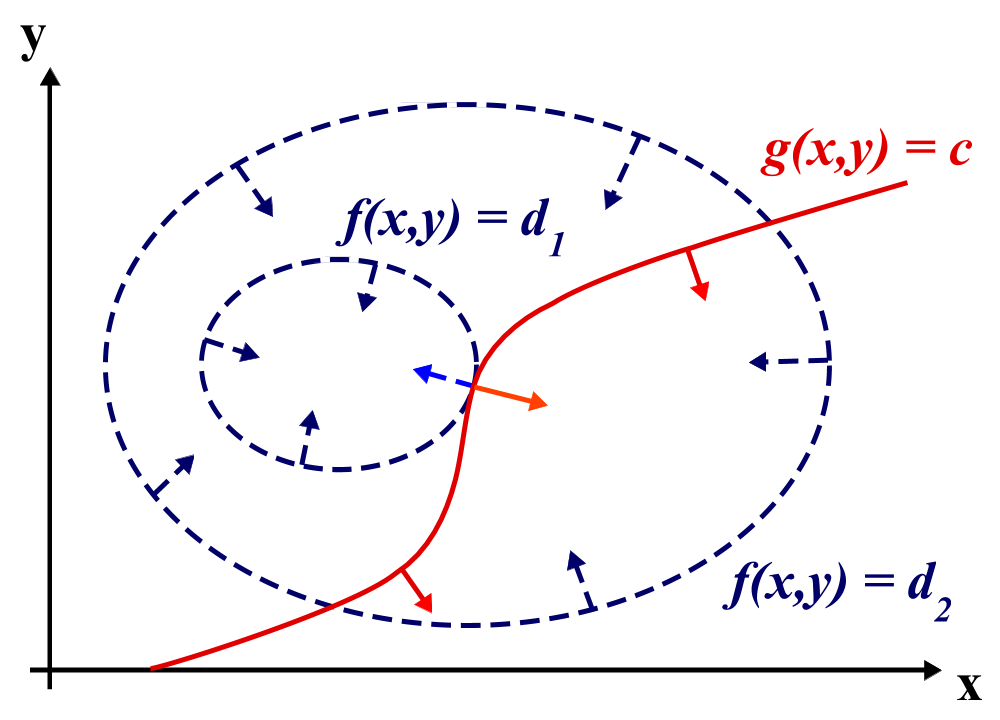
\includegraphics[width=0.5\linewidth]{figs/lagrangian-optimization.png}
\end{center}
If the gradients were not parallel, we could move along $g(x,y)=c$ to a higher contour of $f(x,y)$ by following the component of $\nabla f$ parallel to $g(x,y)=c$.


\newpage
\section{Functional Derivatives}\label{app:functional-derivatives}

A functional is just a function of a function -- i.e.\ some rule $F$ that maps a function $f$ into a number $F[f]$.  Definite integrals are a common example.
In order to optimize a functional $F$ with respect to its argument $f$, one needs to take a \textit{functional derivative}.\footnote{\url{http://en.wikipedia.org/wiki/Functional_derivative}}
To motivate the definition of a functional derivative, first consider the definition of an ordinary derivative
\begin{align}
  \fd{f(x)}{x}
\equiv
  \lim_{\e\rightarrow0}
  \fr{f(x+\e)-f(x)}{\e}
\end{align}
and note the following identity, which you can verify using
$
  f(x+\e)
=
  f(x)
+
  \dfd{f(x)}{x}
  \e
+
  \mc{O}(\e^2)
$.
\begin{align}\label{eq:scalar-derivative-trick}
  \lim_{\e\rightarrow0}
  \fr{f(x+\e)-f(x)}{\e}
=&\
\left.
  \fr{df(x+\e)}{d\e}
\right|_{\e=0}
\end{align}
For multivariate functions, we have the concept of a \textit{directional derivative}
\begin{align}\label{eq:directional-derivative}
  \bo{y}\cdot
  \pd{f(\bo{x})}{\bo{x}}
=
  \lim_{\e\rightarrow0}
  \fr{f(\bo{x}+\e\bo{y}) - f(\bo{x})}{\e}
\end{align}
which measures the change in $f(\bo{x})$ in the direction $\bo{y}$.
Using equation \ref{eq:scalar-derivative-trick}, the directional derivative can be evaluated as an ordinary scalar derivative with respect to $\e$.
\begin{align}\label{eq:vector-derivative-trick}
  \bo{y}\cdot
  \pd{f(\bo{x})}{\bo{x}}
=
  \left.
  \fd{f(\bo{x} + \e\bo{y})}{\e}
  \right|_{\e=0}
\end{align}
The functional derivative $\dfr{\d F}{\d f}$ is defined to satisfy an equation analogous to \ref{eq:directional-derivative}, playing the role of the gradient.
\begin{align}
  \int_{-\infty}^{\infty}
  dx'\,
  g(x')
  \fr{\d F[f]}{\d f(x')}
\equiv
  \lim_{\e\rightarrow0}
  \fr{F[f+\e g] - F[f]}{\e}
\end{align}
This left-hand side could be called a \textit{functional directional derivative}, giving the change in $F$ upon displacing its argument along the function $g$.
Here, the integral takes the role of the dot product in \ref{eq:directional-derivative}.
Using the same trick as in equation \ref{eq:vector-derivative-trick}, the functional derivative can be expressed as an ordinary scalar derivative.
\begin{align}
\label{eq:functional-derivative-trick}
  \int_{-\infty}^{\infty}
  dx'\,
  g(x')
  \fr{\d F[f]}{\d f(x')}
=
  \left.
  \fd{F[f+\e g]}{\e}
  \right|_{\e=0}
\end{align}
The standard procedure for evaluating the functional derivative is to first evaluate the right-hand side of equation~\ref{eq:functional-derivative-trick} for an arbitrary $g$ and then infer what $\dfr{\d F[f]}{\d f(x)}$ must be by comparing to the left-hand side.
Equivalently, $g(x')$ can be replaced with a Dirac delta $\d(x-x')$ in order to arrive at $\dfr{\d F[f]}{\d f(x)}$ directly.

Using eq. \ref{eq:functional-derivative-trick} and the lemma in \cref{app:fundamental-lemma-of-calculus-of-variations}, we find that the stationarity condition for a functional
\begin{align}
  \fr{\d F[f]}{\d f}
\overset{!}{=}
  0
\end{align}
is equivalent to the following condition.
\begin{align}
  \left.
  \fd{F[f+\e g]}{\e}
  \right|_{\e=0}
\overset{!}{=}
  0
&&
  \text{for all $g(x)$}
\end{align}


\newpage
\section{Fundamental Lemma of Calculus of Variations}\label{app:fundamental-lemma-of-calculus-of-variations}
The \textit{Fundamental Lemma of Calculus of Variations}\footnote{\url{http://en.wikipedia.org/wiki/Fundamental_lemma_of_calculus_of_variations}} says that, for continuous functions, the condition
\begin{align}
  \int_{-\infty}^\infty dx f(x)\eta(x)
=
  0
\sp\text{ for all $\eta(x)$}
\end{align}
holds only when $f(x)=0$ for all $x$.
We can see this by considering the case $\eta(x)=f(x)$.
Since $f(x)^2$ is nonnegative everywhere, the integral yields a positive number whenever $f(x)\neq 0$ on a finite range of $x$ values.



\newpage
\section{Unitary Invariances for Hartree-Fock Orbitals}\label{app:hartree-fock-orbital-invariance}

\paragraph{Orthonormality.}
By definition, unitary transformations preserve overlaps.
This can be verified as follows
\begin{align*}
  \ip{\tl\y_i|\tl\y_j}
=
\sum_{kl}
  U_{ki}U_{lj}^*
  \ip{\y_k|\y_l}
=
\sum_{kl}
  U_{ki}U_{lj}^*
  \d_{kl}
=
\sum_k
  U_{ki}U_{kj}^*
=
  \d_{ij}
\end{align*}
using $\sum_k U_{ki}U_{kj}^*=(\bo{U}\bo{U}\dg)_{ji}=(\bo{1})_{ji}=\d_{ji}$.

\paragraph{Fock operator.}
Only the Coulomb and exchange parts of the Fock operator depend on the orbital set.
For the Coulomb part, we have
{\small\begin{align*}
\sum_i
  \ip{\tl\y_i(2)|\op{g}(1,2)|\tl\y_i(2)}
=
\sum_{ijk}
  U_{ji}U_{ki}^*
  \ip{\y_j(2)|\op{g}(1,2)|\y_k(2)}
=
\sum_{jk}
  \d_{jk}
  \ip{\y_j(2)|\op{g}(1,2)|\y_k(2)}
=
\sum_j
  \ip{\y_j(2)|\op{g}(1,2)|\y_j(2)}
\end{align*} \underline{}}%
using the fact that $\sum_i U_{ji}U_{ki}^*=\d_{jk}$.
For the exchange part, we have the same thing with a $\op{P}(1,2)$ sandwiched in there.

\paragraph{Hamiltonian expectation value.}
The vector notation $\bm\y$ for our orbitals allows us to express $\F$ and $\tl\F$ as
\begin{align*}
  \F(1,\ld,n)
=
  \tfrac{1}{\sqrt{n!}}
  |\bm\y(1)\cd\bm\y(n)|
\sp\sp
  \tl\F(1,\ld,n)
=
  \tfrac{1}{\sqrt{n!}}
  |\tl{\bm\y}(1)\cd\tl{\bm\y}(n)|
\end{align*}
which, noting that the matrix $\ma{\tl{\bm\y}(1)\ \cd\ \tl{\bm\y}(n)}$ is simply
\begin{align*}
  \ma{\tl{\bm\y}(1)\ \cd\ \tl{\bm\y}(n)}
=
  \ma{\bo{U}\dg\bm\y(1)\ \cd\ \bo{U}\dg\bm\y(n)}
=
  \bo{U}\dg\ma{\bm\y(1)\ \cd\ \bm\y(n)}
\end{align*}
implies $\tl\F=\det(\bo{U}\dg)\F=\det(\bo{U})^*\F$.
Therefore, $\tl{\F}$ and $\F$ have the same energy expectation values.
\begin{align}
  \ip{\tl\F|\op{H}_e|\tl\F}
=
  \det(\bo{U}\bo{U}\dg)\ip{\F|\op{H}_e|\F}
=
  \ip{\F|\op{H}_e|\F}
\end{align}



\end{document}
